\documentclass[12pt]{report}
\usepackage[utf8]{vietnam}
\usepackage[left=3cm, right=3cm, top=3cm, bottom =3cm]{geometry}
\usepackage{graphicx}
\usepackage{multirow}
\usepackage{array}
\usepackage{fancyhdr}
\usepackage{fancybox}
\usepackage{hyperref}
\usepackage{float}
\usepackage{amsmath}
\usepackage{amssymb}
\usepackage{mathtools}
\usepackage{indentfirst}
\usepackage{caption}
\usepackage{longtable}
\usepackage{lipsum}
\usepackage{enumitem}
\usepackage{booktabs}% http://ctan.org/pkg/booktabs
\newcommand{\tabitem}{~~\llap{\textbullet}~~}

\usepackage{algorithm}
\usepackage{algorithmicx}
\usepackage{algpseudocode}

% Add commands for ceil and floor
\DeclarePairedDelimiter\ceil{\lceil}{\rceil}
\DeclarePairedDelimiter\floor{\lfloor}{\rfloor}

% Add command for argmax
\DeclareMathOperator*{\argmax}{argmax}

% Change name of algorithm
\floatname{algorithm}{Thuật toán}

% set up Input, Output in the algorithm block
\algnewcommand\algorithmicinput{\textbf{Đầu vào:}}
\algnewcommand\INPUT{\item[\algorithmicinput]}
\algnewcommand\algorithmicoutput{\textbf{Đầu ra:}}
\algnewcommand\OUTPUT{\item[\algorithmicoutput]}

% Specify depth to show in then table of contents
% -1 part   1 section       3 subsubsection     5 subparagraph
% 0 chapter 2 subsection    4 paragraph
\setcounter{tocdepth}{4}

% Specify depth to show in document
\setcounter{secnumdepth}{3}

% Link color setup
\hypersetup{
	colorlinks = true,
	linkcolor = black,
	citecolor = blue
}

% Change format of page
\pagestyle{fancy}
\fancyhf{}
\fancyhead{}
\fancyfoot{}
\fancyhead[L]{Bài tập lớn - Cơ sở dữ liệu}
\fancyfoot[L]{Đề tài: "DataTone: Managing Ambiguity in Natural Language Interfaces for Data Visualization"}
\fancyfoot[R]{\thepage}
\renewcommand{\headrulewidth}{1pt}
\renewcommand{\footrulewidth}{1pt}

% \patchcmd{\chapter}{\thispagestyle{plain}}{\thispagestyle{fancy}}{}{}

\renewcommand{\thesection}{\arabic{section}}
\renewcommand{\thesubsection}{\thesection.\arabic{subsection}}
\renewcommand{\thesubsubsection}{\thesubsection.\arabic{subsubsection}}

% format
\usepackage{titlesec}
\usepackage{etoolbox}
\makeatletter
\patchcmd{\ttlh@hang}{\parindent\z@}{\parindent\z@\leavevmode}{}{}
\patchcmd{\ttlh@hang}{\noindent}{}{}{}
\makeatother

\titleformat{\subsection}
{\normalfont\large\bfseries}{\thesubsection}{1em}{}
\titleformat{\subsubsection}
{\normalfont\large\sffamily\bfseries}{\thesubsubsection}{1em}{}

% tab command
\newcommand\tab[1][1cm]{\hspace*{#1}}

\begin{document}

%%%%%%%%%%%%%%%%%%%%%%%%% Title Page %%%%%%%%%%%%%%%%%%%%%%%%%%%%%
\thispagestyle{empty}
\thisfancypage{\setlength{\fboxsep}{0pt}\fbox}{}

\begin{center}
\begin{large}
TRƯỜNG ĐẠI HỌC BÁCH KHOA HÀ NỘI
\end{large} \\
\begin{large}
VIỆN CÔNG NGHỆ THÔNG TIN VÀ TRUYỀN THÔNG
\end{large} \\
\textbf{--------------------  *  ---------------------}\\[2.3cm]
{\fontsize{32pt}{1}\selectfont BÁO CÁO THU HOẠCH}\\
{\fontsize{20pt}{1}\selectfont BÀI BÁO}\\[0.5cm]
{\fontsize{18pt}{1}\selectfont "DataTone: Managing Ambiguity in Natural Language Interfaces for Data Visualization"}\\[0.5cm]

\includegraphics[width=4cm]{hust.jpg}\\[1.3cm]
\end{center}

\hspace{2.5cm} Nhóm sinh viên thực hiện: \hspace{4pt}
\textbf{\parbox[t]{5cm}{    
    Nguyễn Quang Quý \\
    Tạ Bảo Thắng
}}\\[12pt]

\hspace{2.5cm} Giáo viên hướng dẫn \hspace{24pt}:  \hspace{4pt} \textbf{\parbox[t]{5cm}{    
TS Nguyễn Kim Anh
}}

\vspace{1.5cm}
\begin{center}
{\fontsize{14pt}{1}\selectfont HÀ NỘI}\\
{\fontsize{14pt}{1}\selectfont \today}
\end{center}
\pagenumbering{gobble}
\tableofcontents 
\newpage
\listoftables
\newpage
\listoffigures
\newpage

\pagenumbering{arabic}
\newpage
\setcounter{page}{1}

\section{Vấn đề được giới thiệu trong bài báo}
\paragraph*{}
Phân tích dữ liệu là một công việc khó, với sự hỗ trợ của các công cụ để biểu thị dữ liệu như Microsoft Exel, Tableau, … Nhưng để trả lời cho những câu hỏi tinh vi, yêu cầu người dùng phải có hiểu biết về các công cụ dành cho chuyên gia phân tích. Nhưng có một cách dễ dàng hơn để giải quyết điều này đó là sử dụng giao diện ngôn ngữ tự nhiên. Người dùng có thể đặt câu hỏi trực tiếp mà không cần học các công cụ hoặc cách chuyển câu hỏi của họ thành trang tính hoặc các thao tác hiển thị dữ liệu. Tuy nhiên, ngôn ngữ tự nhiên thường tồn tại với những nhập nhằng, và sự nhập nhằng thể hiện ở nhiều mức :
\begin{itemize}
	\item thứ nhất, câu hỏi của người dùng có thể sẽ không được 	xác định. \\
	Ví dụ: khi người trong câu hỏi có từ  “product”, và trong CSDL tồn tại “product category” và “product name” khi đó “product” sẽ tương ứng với cụm từ nào ?
	
	\item thứ hai, có thể có nhiều câu trả lời cho câu hỏi của nguời dùng. \\
	Ví dụ:“show revenue for New York City and Washington DC in 2012.” \\
	Mục đích câu hỏi là so sánh tổng GDP của NYC các năm với WDC năm 2012 hay cả hai thành phố này đều trong năm 2012 ?
\end{itemize}
Thậm chí khi sự nhập nhằng về mặt ngôn ngữ được giải quyết, thì chúng ta cũng cần lựa chọn được cách biểu thị dữ liệu cho phù hợp:
\begin{itemize}
	\item biểu đồ thanh chồng nhau: x- thời gian, y- mỗi khối ứng với 1 thành phố
	\item 2 biểu đồ cột, mỗi cột ứng với một thành phố
	\item biểu đồ đường - mỗi đường ứng với một thành phố
	\item ...
\end{itemize}
Có nhiều hệ thống đã được thiết kế để có thể giải quyết được vấn đề này như IBM Watson Analytics, Microsoft Power BI, ...Nhưng hạn chế của các hệ thống này là ràng buộc người dùng với một tập mẫu câu hỏi đã được lược bỏ đi sự nhập nhằng để cho hệ thống có thể hiểu được, điều đó làm mất đi sự toàn vẹn trong câu truy vấn của người dùng. Trong bài báo này, đã đề xuất một hệ thống mới có tên DataTone cho phép giữ lại sự toàn vẹn trong câu truy vấn của người dùng. 
\paragraph*{}
Cách thức hệ thống DataTone hoạt động: người dùng nhập vào câu truy vấn ngôn ngữ tự nhiên , hệ thống phân tích truy vấn và tạo một hoặc nhiều đặc tả dữ liệu (DSP) dùng để tạo ra truy vấn đối với CSDL. Từ DSP và truy vấn đối với CSDL, DataTone tạo các đặc tả trực quan (VSP) và tạo các biểu diễn tương ứng. Hệ thống sẽ xếp hạng các biểu diễn được tạo ra và trả về biểu diễn có rank cao nhất cho người dùng. Sự nhập nhằng được giải quyết nhờ vào sự kết hợp giữa điều khiển của người dùng và điều khiển của hệ thống. Bài báo đưa ra một khái niệm “ambiguity space” để nói đến mô hình của sự nhập nhằng xuất hiện trong mỗi bước của đường ống trên. Tương tác với “ambiguity space” thông qua “ambiguity widget” - cho phép người dùng điều chỉnh quyết định của hệ thống trong quá trình tạo ra biểu thị. \\
Đóng góp của bài báo:
\begin{itemize}
	\item Một phương pháp tiếp cận khởi tạo hỗn hợp cho phép người dùng tạo biểu thị dữ liệu của câu trả lời từ câu truy vấn tự nhiên,	\item ambiguity space - mô hình của sự nhập nhằng trong truy vấn ngôn ngữ tự nhiên cho khám phá và biếu thị dữ liệu,
	\item thiết kế giao diện bao gồm các ambiguity widget, cho phép người dùng cung cấp các phản hồi tới hệ thống để xử lý nhập nhằng và điều hướng “ambiguity space”
	\item thuật toán quản lý các chỉnh sửa nhập nhằng theo thời gian qua các ràng buộc ưu tiên,
	\item thiết kế nghiên cứu mới để đánh giá các giao diện ngôn ngữ tự nhiên cho phân tích dữ liệu.
\end{itemize}
%end section one
\section{Giao diện của hệ thống DataTone}
\begin{figure}[h]
	\centering
	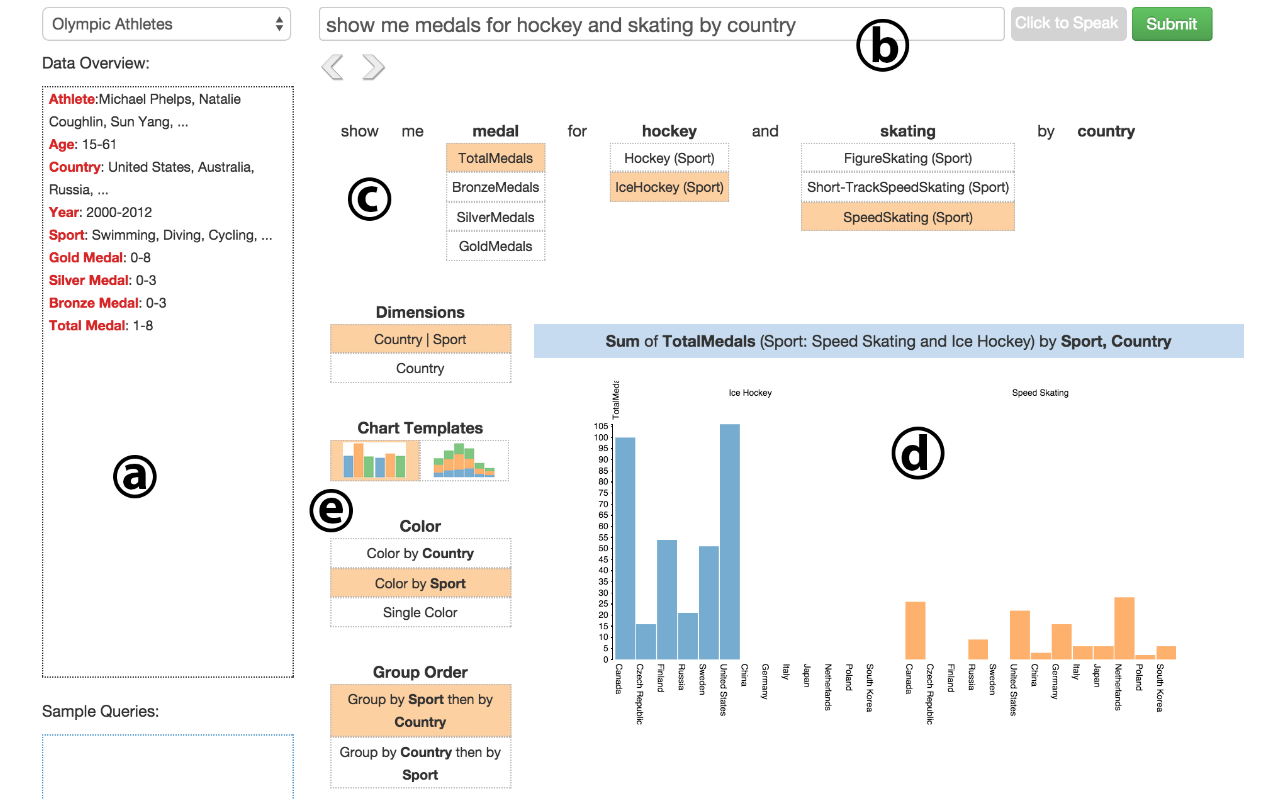
\includegraphics[width=20cm,
	height=9cm, keepaspectratio]{DataToneGUI.png}
	\caption{Giao diện người dùng của hệ thống DataTone}
\end{figure}
Trên hình là giao diện người dùng của hệ thống DataTone , bao gồm 4 phần :
\begin{itemize}
	\item Tổng quan dữ liệu: mô tả khái quát các thuộc tính có trong tập dữ liệu được chọn.
	\item Hộp nhập truy vấn: người dùng có thể nhập từ bàn phím hoặc bằng giọng nói.
	\item Biểu thị: Biểu đồ mô tả câu trả lời cho truy vấn.
	\item Widget: Những option hệ thống đề xuất cho người dùng để tăng tính đúng đắn của câu trả lời mà người dùng mong muốn.
\end{itemize}
Ví dụ : truy vấn “show me  medals for hockey and skating by country” \\
Hệ thống ghi nhận được 3 nhập nhằng dữ liệu tồn tại: 
\begin{itemize}
	\item Medals: tổng số hay chỉ gold hoặc chỉ silver hay chỉ bronze
	\item hockey:  Hockey(Sport ) hay IceHockey(Sport)
	\item Skating
\end{itemize}


\section{Hệ thống DataTone}
\begin{figure}[h!]
	\centering
	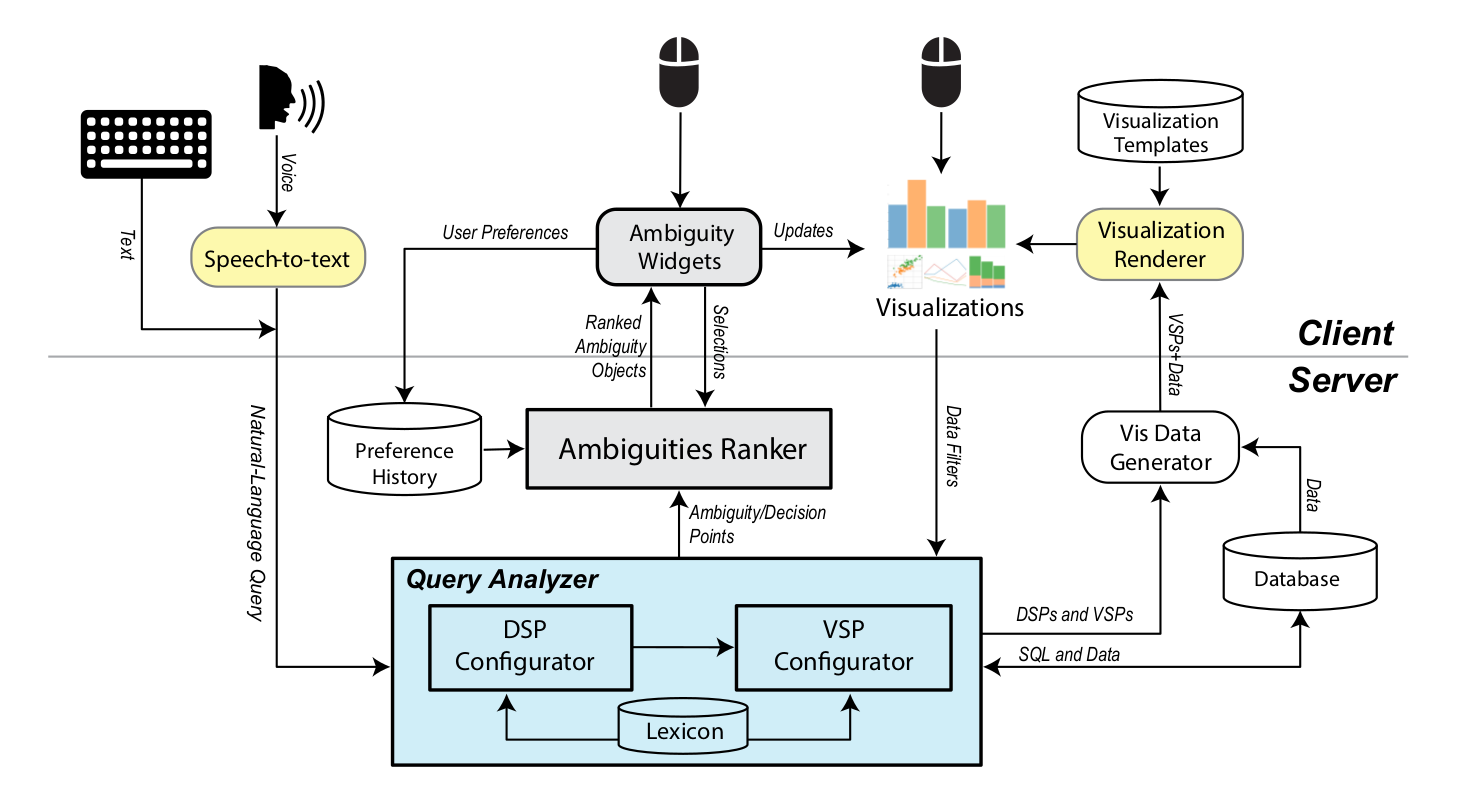
\includegraphics[width=15cm, height=8cm]{DataToneSystem.png}
	\caption{Kiến trúc hệ thống DataTone}
\end{figure}
Trong hệ thống DataTone, Query Analyzer có chức năng là chuyển đổi từ câu truy vấn sử dụng ngôn ngữ tự nhiên sang hai định dạng trung gian:
\begin{itemize}
	\item Data Specification (DSP): capture những khía cạnh liên quan tới dữ liệu của truy vấn đầu vào và truy vấn đối với CSDL.
	\item Visual Specification (VSP): là một ngữ pháp đồ họa dùng để ánh xạ các thành phần của DSP với những thông tin cần thiết trong việc render các view. 
\end{itemize}
\subsection{Natural language interpretation}
\subsubsection{Tokenization and similarity mapping}
Để chuyển đổi giữa ngôn ngữ tự nhiên và biểu thị trực quan , DataTone thực hiện một số chuyển đổi , đầu tiên sẽ ánh xạ ngôn ngữ tự nhiên với DSP , sau đó là DSP với VSP. \\
Ban đầu cần xác định được các đặc trưng bậc thấp của ngôn ngữ tự nhiên (ví dụ :từ , cụm từ, ...) có nghĩa trong ngữ cảnh của tập dữ liệu và các tác vụ phân tích. Tập các cụm từ đó được tạo ra bằng cách lấy tất cả n-gram của câu. Sau đó xác định những n-gram liên quan tới tập dữ liệu và định nghĩa tác vụ bằng cách so sánh mỗi n-gram với tập biểu thức chính quy và một từ điển gồm các cụm từ phổ biến (ví dụ: "compare", "average", "less than"). Cụ thể,hệ thống thực hiện gắn mỗi n-gram với một trong 8 nhãn :
\begin{itemize}
	\item database attributes
	\item database cell values
	\item numerical values
	\item time expressions
	\item data operators and functions (ví dụ: greater than, less than, equal, sum, average, sort)
	\item visualization key phrases (ví dụ: trend, correclation, relationship, distribution, time series , bars, stacked bars, line graph)
	\item conjunction and disjunction terms (ví dụ and , or)
	\item “direct manipulation” terms (ví dụ : add, color)
\end{itemize}
Những n-gram được gắn chính xác với một từ vựng hoặc mẫu biểu thức chính quy được gắn nhãn tự động. Ngược lại, việc gắn nhãn sẽ dựa trên sự tương đương về mặt ngữ nghĩa thông qua việc đánh giá  t = Sim($ngram_{i}$, $lexicon_{j}$). Nêú t > 0.8 thì cặp ( $ngram_{i}$, $lexicon_{j}$ ) sẽ được lựa chọn: \\
Sim($ngram_{i}$, $lexicon_{j}$ )=MAX\{$Sim_{wordnet}$ (. . . ), $Sim_{spelling}$ (. . . )\}.
\begin{itemize}
	\item $Sim_{wordnet}(ngram_{i}, lexicon_{j})$: khoảng cách đồ thị trong đồ thi worldNet
	\item $Sim_{spelling}(ngram_{i}, lexicon_{j})$ = $\dfrac{\vec{ngram_{i}}.\vec{lexicon_{j}}}{den}$: xử lý các lỗi chính tả chính bằng cách kiểm tra sự tương tự "bag of words" trong 2 token
\end{itemize}

\subsubsection{Relation identification}
Sau khi đã gắn nhãn, xây dựng bộ lọc bằng Stanford Core NLP Parser để tạo cây phân tích ngữ nghĩa và ngữ pháp.
\paragraph*{Ví dụ:}
 ”show me the states that had total sales greater than than 20000 and less than 100000”
 \\
 Ngữ pháp : “total sales” :NP (noun phrase), “greater than 20000 “ :ADJP (adjective phrase)
 \\
 Ngữ nghĩa: “greater than” and “less than” are connected to total sales.
 
\subsection{Data specification (DSP)}
Từ sự phân tích và gắn nhãn có thể tạo ra một hoặc nhiều DSP. Các thuộc tính trong DSP bao gồm:
\begin{itemize}
	\item Attributes: giữ lại các thuộc tính được xác đinh trong câu gốc 
	\item Values: dạng string, number, time, … được xác định trong câu
	\item Filters 
	\item Order: thứ tự xắp sếp dữ liệu được xác trong câu truy vấn
	\item Aggregates: sums, averages, maximum values, counts, ...
	\item Dimensions: biến độc lập - cách phân vùng dữ liệu
	\item Measures: đơn vị tính toán 
\end{itemize}
Sau đó câu lệnh truy vấn CSDL được tạo theo dạng:\\
SELECT \{Aggregates\}, \{Dimension Attributes\} FROM Table WHERE \{Implicit Filters\} GROUP BY \{Dimension Attributes\} HAVING \{Explicit Filters\} ORDER BY \{Order\}
\subsection{Visualization generation}
\paragraph*{}
Kết quả thu được từ truy vấn SQL cùng với DSP đã tạo ra sẽ được sử dụng để tạo ra VSP (visual specification) cho mỗi DSP. Nếu truy vấn SQL không trả về kết quả hoặc dữ liệu trong kết quả quá ít thì hệ thống sẽ bỏ qua DSP đó. DataTone hiện tại hỗ trợ một số lượng hữu hạn loại biểu thị (scatter plots, various bar and line chart formats). Mỗi lọai được đại diện bởi VSP "template" khác nhau ứng với các cấu hình khác nhau. Hệ thống sử dụng thư viện D3.js để render VSP được trả về cho client.
\paragraph*{}
DataTone cố gắng ánh xạ mỗi DSP với mẫu VSP ứng với cấu hình cụ thể của DSP (dựa trên measure, dimension và loại DSP). Điều này có nghĩa là nhiều VSP có thể phù hợp với DSP đã cho. VSP được xếp hạng từ cao tới thấp và giúp cho người dùng dễ dàng xử lý sự nhập nhằng thông qua sự tương tác đơn giản với widget.
\section{Xử lý sự nhập nhằng}
\begin{figure}[h!]
	\centering
	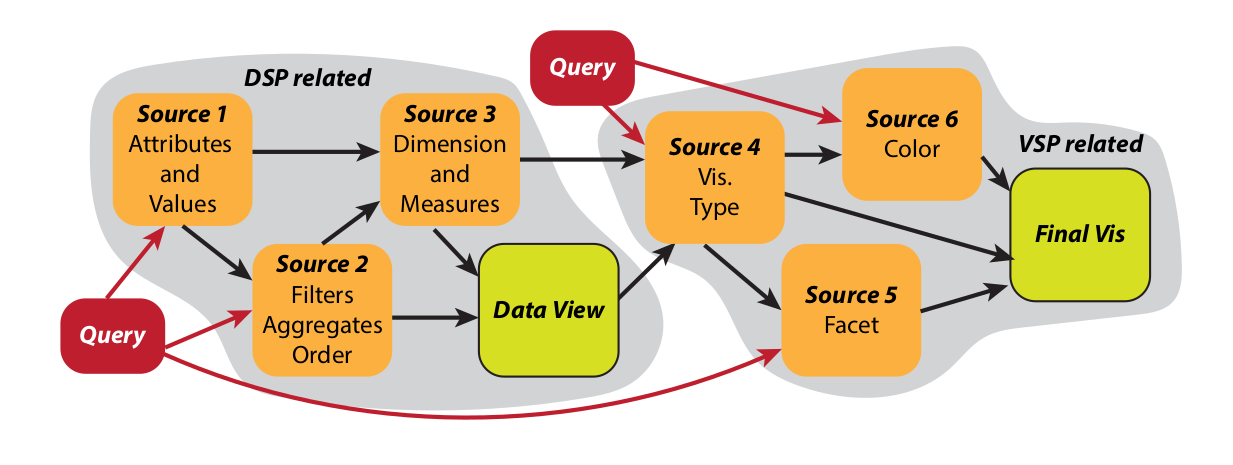
\includegraphics[width=15cm, height=6cm]{Ambiguity.png}
	\caption{Những sự phụ thuộc trong "Ambiguity space"}
\end{figure}

Các phần tử đường ống khác nhau trong DataTone tạo ra các loại nhập nhằng khác nhau, từ đó có thể dẫn đến nhiều sự biểu diễn khác nhau cho một truy vấn. Để biểu thị kết quả cho người dùng, lựa chọn đơn giản là hiển thị tất cả các biểu diễn khác nhau cho truy vấn đó. Tuy nhiên, sự nhập nhằng tăng theo cấp số nhân, do vậy không thể giải quyết như vậy được. DataTone xử lý bằng cách xếp hạng các VSP và cung cấp cho người dùng cuối  một kĩ thuật đẻ chuyển đổi nhanh chóng giữa các biểu thị.

\subsection{Sự nhập nhằng dữ liệu}
Sự nhập nhằng ngôn ngữ có thể xuất hiện ở mức từ vựng hoặc cú pháp.Sự mơ hồ từ vựng phát sinh do đa nghĩa và sự mơ hồ cú pháp do các cấu trúc có thể của câu .Việc tạo thành nhiều lời giải thích có thể của truy vấn dẫn đến nhiều nguồn nhập nhằng .
\subsubsection*{Source 1: Nhận diện thuộc tính cơ sở dữ liệu và giá trị văn bản} 
Người dùng cuối thường liên hệ tới các thực thể và các thuộc tính trong nhiều cách mơ hồ.
\\
Ví dụ: khi người dùng hỏi về “product" và trong CSDL đang có thông tin về “product category“ và “product sub-category”, vậy thì thuộc tính nào sẽ được ánh xạ ?
\\
DataTone xử lý vấn đề này bằng cách tính toán hàm Sim đã nhắc tới ở trên.
\subsubsection*{Source 2: Nhận diện các bộ lọc, phân loại và tổng hợp}
Một câu truy vấn có thể được phân tích theo nhiều dạng cú pháp, dẫn đến nhiều dạng cấu trúc của câu đối với cùng một truy vấn.
\\
Ví dụ: “population in Michigan and California in 2012” có thể được phân tích như một yêu cầu cho dân số của Michigan hiện tại và California năm 2012  thay vì cả 2 bang đều năm 2012. DataTone xử lý bằng cách dùng các bộ lọc tường minh.
\subsubsection*{Source 3: Lựa chọn Dimension và measure} 
Khi người dùng xác định bộ lọc, không rõ liệu có nên xử lý các thuộc tính của một bộ lọc như là một thuộc tính dimension hay không. Hệ thống có thể xếp hạng các option một cách heuristic, những thuộc tính dạng số thường là measure và những thuộc tính phân loại thường là dimension. Với một số trường hợp mà biến phân loại gồm quá nhiều trường hợp duy nhất, DataTone tính toán các giá trị duy nhất khác biệt chia cho số hàng. Kết quả thu được là cao thì sẽ quyết định xử lý cột đó như một measure (theo tính toán giá trị ngưỡng nhỏ nhất là 0.7)
\subsection{Sự nhập nhằng trong quyết định thiết kế}
\subsubsection*{Source 4: Lựa chọn mẫu biểu thị}
Cho một DSP, có thể sẽ tồn tại nhiều mẫu VSP. DataTone sử dụng trực tiếp các lệnh trực tiếp hoặc các định nghĩa nhiệm vụ.Thực hiện điều này thông qua việc sử dụng từ điển. Tập từ điển của DataTone bao gồm các từ liên quan tới 4 tác vụ : comparison, correlation, distribution analysis và trends. 
\subsubsection*{Source 5: Faceting data for small multiples} 
Các hiển thị small-multiple của thông tin giúp cho việc so sánh dữ liệu và tìm mẫu thông quan nhiều chiều. Với truy vấn đề cập đến nhiều thuộc tính dữ liệu, sự nhập nhằng đến từ quyết định thuộc tính nào để sử dụng như các tham số khía cạnh cho các bội số nhỏ và cách tổ chức chúng. Từ tập VSP đã xếp hạng, hệ thống ưu tiên  xếp hạng nhóm phù hợp với thứ tự trong các thuộc tính được đề cập trong truy vấn. 
\subsubsection*{Source 6: Chọn phương pháp mã hóa} 
Màu sắc, hình dạng, và kích thước là các biến phổ biến trong một biệu thị. Trong mẫu thử nghiệm hiện tại, DataTone chỉ hỗ trợ mã hóa màu. Tuy nhiên, có thể vẫn còn mơ hồ trong việc sử dụng màu hay không. Mặc dù màu sắc có thể không được gọi rõ ràng, hoặc có thể dẫn đến mã hoá kép, nó vẫn có thể được mong muốn.

\section{Đánh giá}

\begin{itemize}
	\item Để đánh giá DataTone, tác giả đã tiến hành một nghiên cứu so sánh đánh giá của người dùng với hệ thông Watson của IBM.
	\item So sánh 2 hệ thống Watson và DataTone:
		\begin{itemize}
			\item Giống: cho phép người dùng xây dựng các hình ảnh hóa thông qua sự kết hợp giữa:
				\begin{itemize}
					\item Tương tác ngôn ngữ tự nhiên. 
					\item Thao tác trực tiếp.
				\end{itemize}
			\item Khác: Cách chúng tiếp cận sự mơ hồ:
				\begin{itemize}
					\item DataTone:  xây dựng một hình ảnh trực quan trực tiếp từ truy vấn của người dùng.
					\item Watson: Đáp ứng truy vấn của người dùng bằng 1 danh sách các câu hỏi được đề xuất ( các câu hỏi mà hệ thống có thể trả lời bằng hình ảnh trực quan dữ liệu), sau đó mới cho người dùng điều chỉnh hình ảnh tạo ra thông qua thao tác trực tiếp.
				\end{itemize}
		\end{itemize}
	\item Do 2 hệ thống khác nhau về thiết kế giải quyết sự mơ hồ trong ngôn ngữ tự nhiên, nên tác giả quyết định sẽ so sánh toàn diện 2 hệ thống thay vì so sánh từng thành phần riêng lẻ.
	\item Phương pháp đánh giá:  Đánh giá Jeopardy :
		\begin{itemize}
			\item Đánh giá Jeopardy  lấy cảm hứng từ  một gameshow trên truyền hình của Mỹ. Ớ đó người dùng sẽ phải đưa ra câu trả lời dưới định dạng 1 câu hỏi.
			
			\item Người chơi phải đưa ra câu trả lời bằng  các hình ảnh trực quan  để chứng minh đúng đắn hay phủ định điều đó.
			
			\item Ví dụ:  Chúng ta có thể nói rằng: “North Vietnam has the fewest number of people without jobs”
			
			\item Người chơi  phải đưa ra sự đúng sai của nhận định đó bằng cách sử dụng hệ thống để chứng minh nó bằng hình ảnh trực quan. Người chơi có thể sử dụng  DataTone hoặc Watson cho đến khi họ tin rằng họ đã đạt được một câu trả lời thỏa đáng. 
			
			\item Tác  giả chọn các chủ đề sao cho nếu người chơi chỉ đơn giản là lặp lại các từ ngữ trong chủ đề 1 cách đơn giản sẽ không thể tạo ra được 1 view chính xác.
			
			\item Một câu trả lời hợp lí cho chủ đề nêu ở ví dụ trên là  “Show me a sorted view of unemployment by state”
			\item Trong khảo sát, tác giả khảo sát 16 người tham gia, trong thời gian 1h với 3 bộ Dataset, 10 chủ đề /dataset
			\item 14/16 người thích sử dụng DataTone hơn.
		\end{itemize}
\end{itemize}

\textbf{Kết quả khảo sát}
\begin{figure}[h]
	\centering
	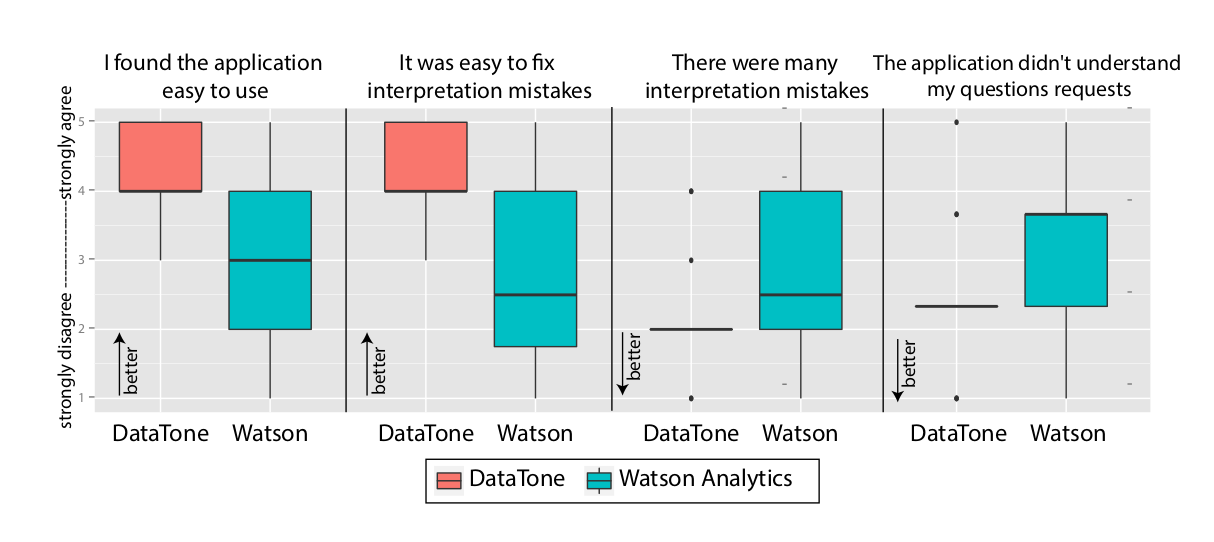
\includegraphics[width=20cm,
	height=6cm, keepaspectratio]{Result.png}
	\caption{So sánh DataTone và IBM Waston}
\end{figure}
\section{Thảo luận và công việc trong tương lai}
\begin{itemize}
	\item Hệ thống DataTone tốt hơn các sản phẩm thương mại hiện đại trên rất nhiều mẫu.
	
	\item Hệ thống có 1 vài hạn chế như:
		\begin{itemize}
			\item Sự phân giải mơ hồ dựa vào heuristic
			
			\item Linh hoạt hơn các  widget trừu tượng
			 
			\item Hiện tại, tác giả chỉ hỗ trợ các bộ dữ liệu bảng đơn.
			
			\item Cuối cùng, mặc dù DataTone cung cấp đầu vào giọng nói, nhưng nó chưa khuyến khích được dùng do chưa hoàn thiện
			
		\end{itemize}
	
\end{itemize}

\end{document}
